\chapter{Architettura della piattaforma}
\label{sec:architettura}

La piattaforma si compone di due componenti principali: un Flight Controller basato su ESP32 e un Server che opera in ambiente desktop Windows. Entrambi i componenti interagiscono tramite rete WiFi, utilizzando protocolli come mDNS per la scoperta dei dispositivi e HTTP per la trasmissione dei dati. Questa architettura garantisce un sistema integrato e scalabile per il controllo di un aeromobile, offrendo funzionalità di monitoraggio remota e raccolta di dati.

\begin{itemize}
\item \textbf{Flight Controller:} gestisce le operazioni di volo, tra cui acquisizione dei dati dai sensori, elaborazione in tempo reale e controllo degli attuatori.
\item \textbf{Server:} fornisce funzionalità di logging remoto, monitoraggio e interfaccia utente.
\item \textbf{Comunicazione ESP32-Server:} utilizza WiFi per sincronizzazione e scambio dati.
\end{itemize}

\begin{figure}[h!]
    \centering
    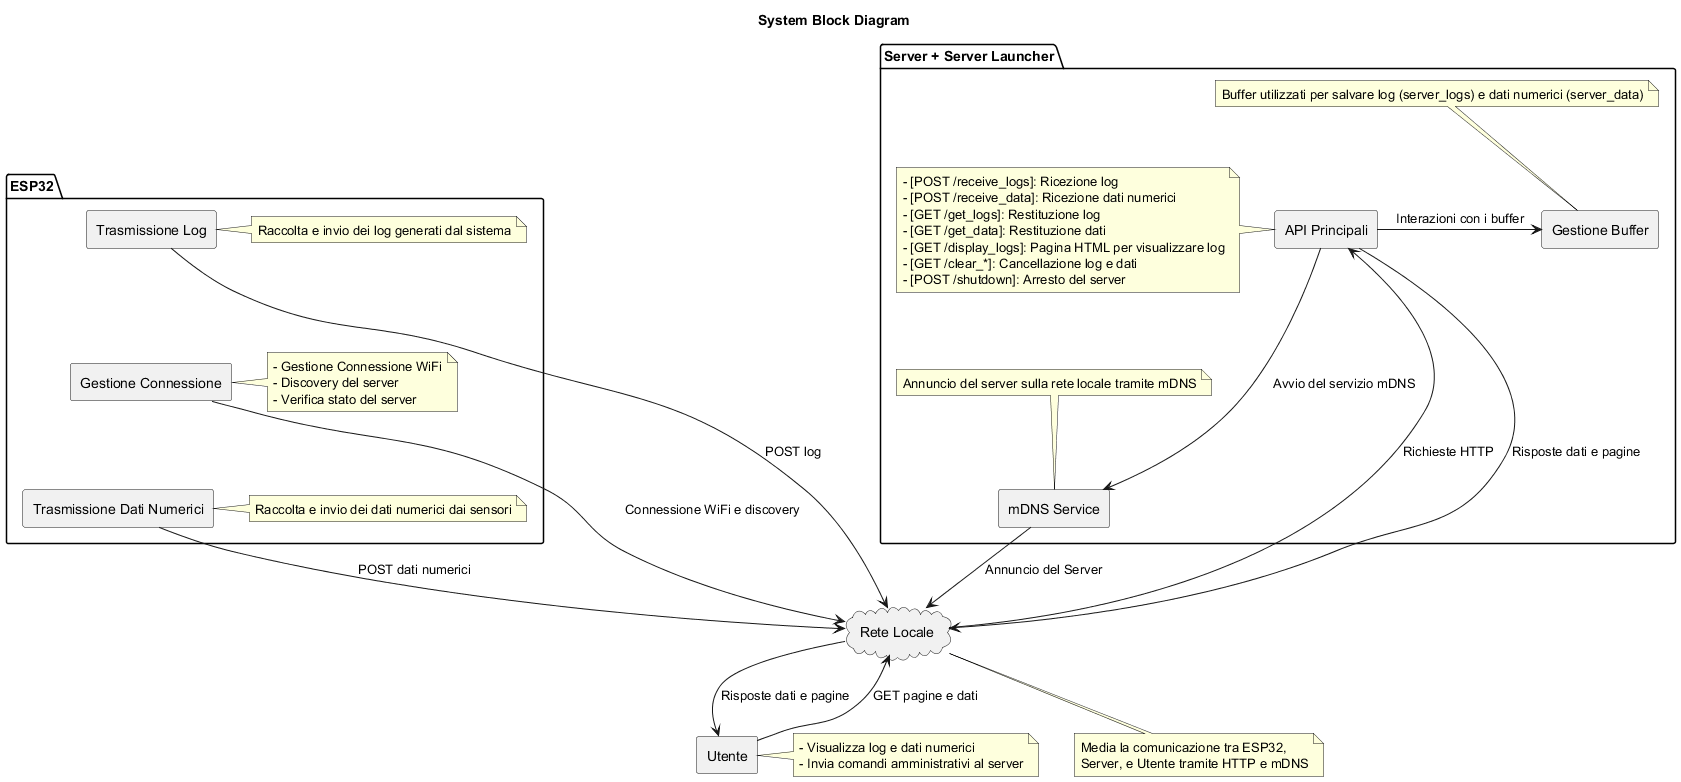
\includegraphics[width=]{diagrams/system_block_diagram.png}
    \caption{Diagramma a blocchi del sistema.}
    \label{fig:system_block_diagram}
\end{figure}

\begin{figure}[h!]
    \centering
    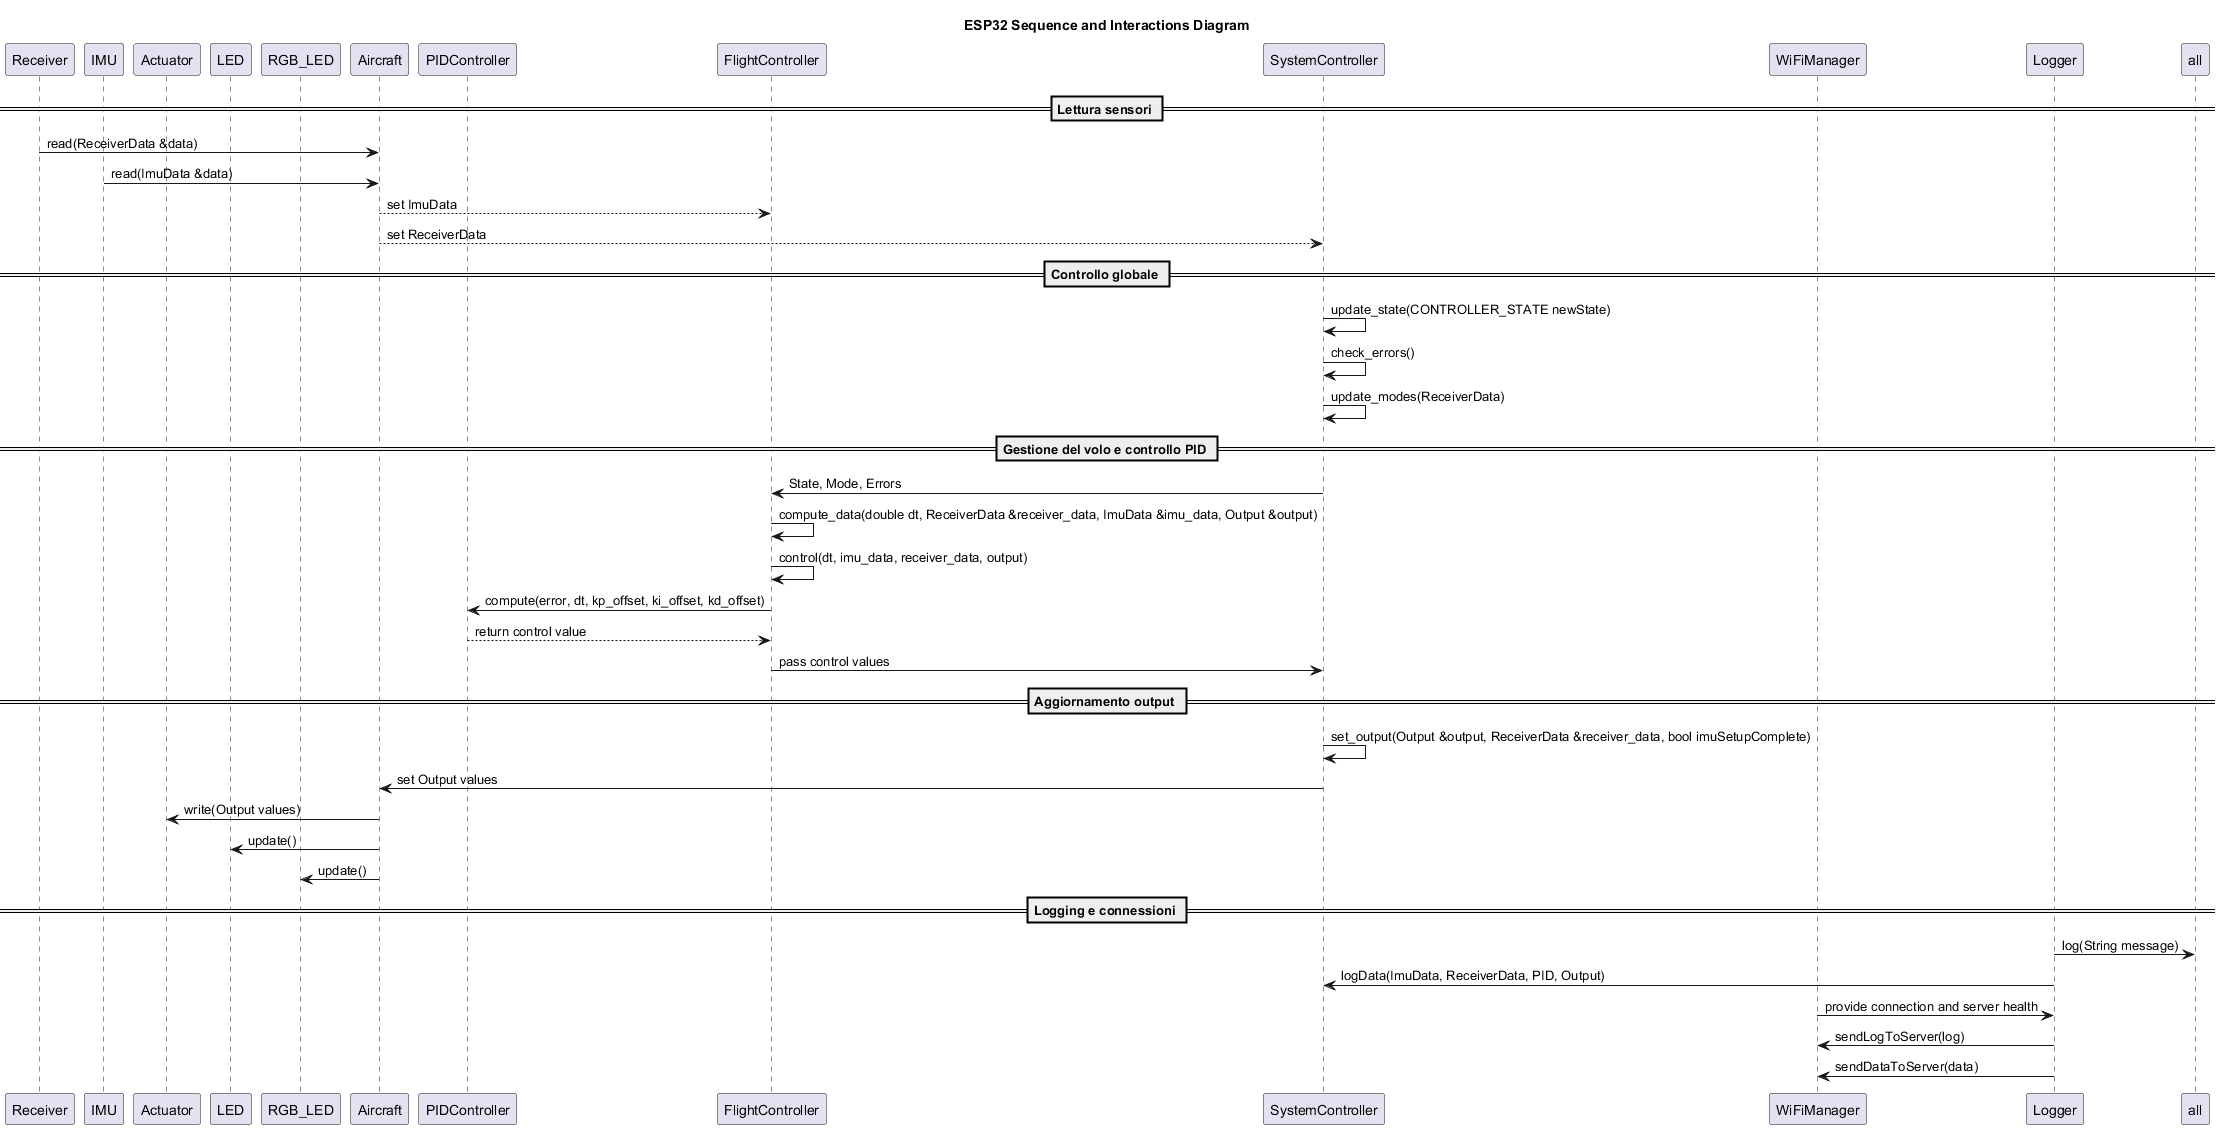
\includegraphics[width=\textwidth]{diagrams/esp32_interactions.png}
    \caption{Diagramma delle interazioni ESP32-Server.}
    \label{fig:esp32_interactions}
\end{figure}


\section{Architettura del server}
Il server è progettato per ricevere e gestire i dati provenienti dal Flight Controller, offrendo un'interfaccia per l'analisi e la gestione remota.

\subsection{Componenti principali del server}
\begin{itemize}
\item \textbf{Moduli di logging:} raccolgono e archiviano dati diagnostici inviati dalla ESP32.
\item \textbf{Comunicazione:} implementa protocolli come HTTP e mDNS per la scoperta e lo scambio di dati.
\item \textbf{Interfaccia utente:} consente la visualizzazione dei dati in tempo reale tramite browser.
\end{itemize}

\begin{figure}[h!]
    \centering
    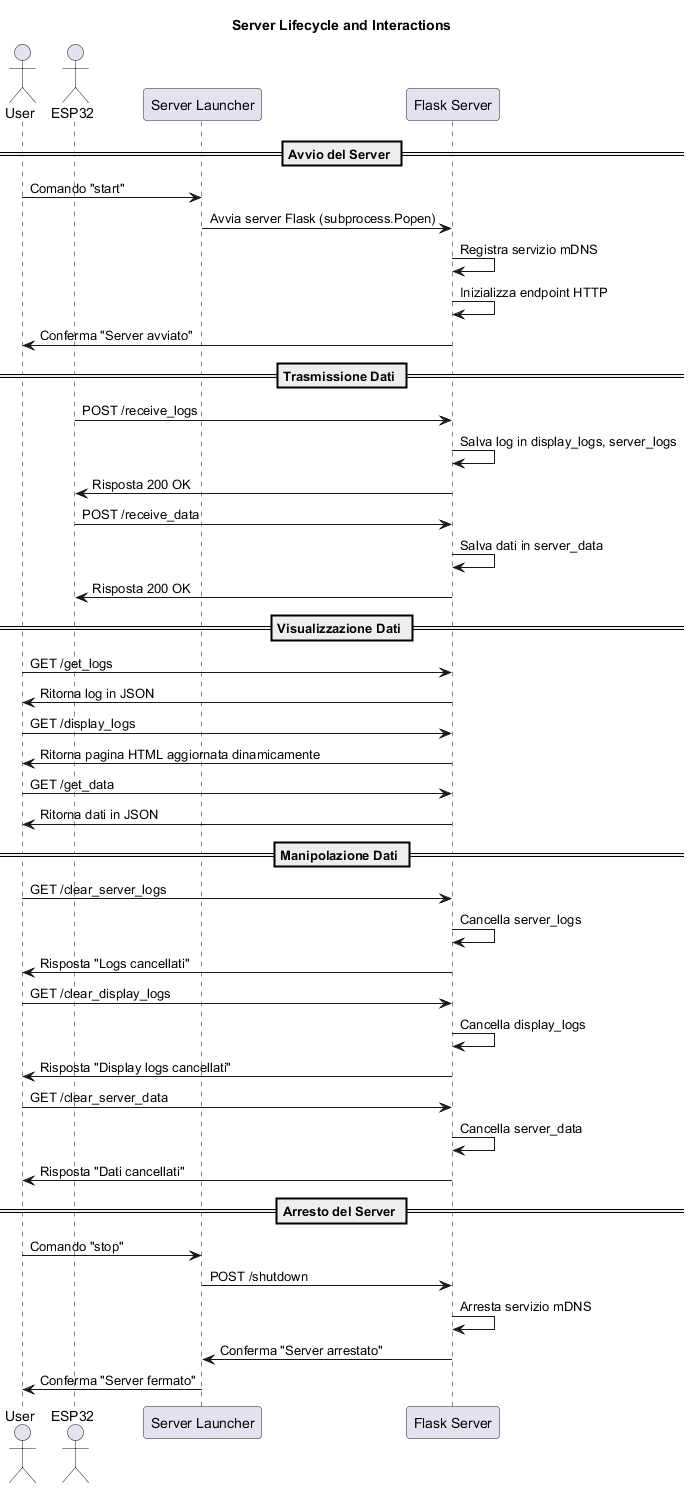
\includegraphics[width=\textwidth]{diagrams/server_lifecycle_interactions.png}
    \caption{Diagramma delle interazioni del server.}
    \label{fig:server_lifecycle_interactions}
\end{figure}


\section{Architettura del software di volo}
Il software di volo, in esecuzione su ESP32, è responsabile della stabilità e del controllo dell'aeromobile. L'architettura è orientata agli oggetti per garantirne la modularità.

\subsection{Blocchi funzionali del software}
\begin{itemize}
\item \textbf{Input:}
\begin{itemize}
\item Acquisizione e validazione dei dati dai sensori IMU e dal ricevitore.
\item Mappatura dei dati grezzi in formati utilizzabili per il controllo.
\end{itemize}
\item \textbf{Elaborazione:}
\begin{itemize}
\item Verifica e gestione degli errori.
\item Aggiornamento dello stato e delle modalità operative.
\item Calcolo PID per stabilizzazione giroscopica e controllo attitudine.
\end{itemize}
\item \textbf{Output:}
\begin{itemize}
\item Scrittura dei valori sugli attuatori per il controllo dei motori.
\item Aggiornamento dei LED per feedback visivo.
\end{itemize}
\item \textbf{Logging:}
\begin{itemize}
\item Raccolta e trasmissione di dati diagnostici al server.
\item Formattazione dei messaggi di log.
\end{itemize}
\item \textbf{Comunicazione:}
\begin{itemize}
\item Configurazione della rete WiFi.
\item Scoperta del server tramite mDNS.
\item Sincronizzazione dei dati in tempo reale.
\end{itemize}
\end{itemize}

\subsection{Classi principali}
\begin{itemize}
\item \textbf{Componenti fisiche:} Actuator, Receiver, IMU, LED.
\item \textbf{Componenti logiche:} Aircraft, FlightController, PIDController, SystemController.
\end{itemize}

\subsection{Diagrammi principali}
\begin{figure}[h!]
    \centering
    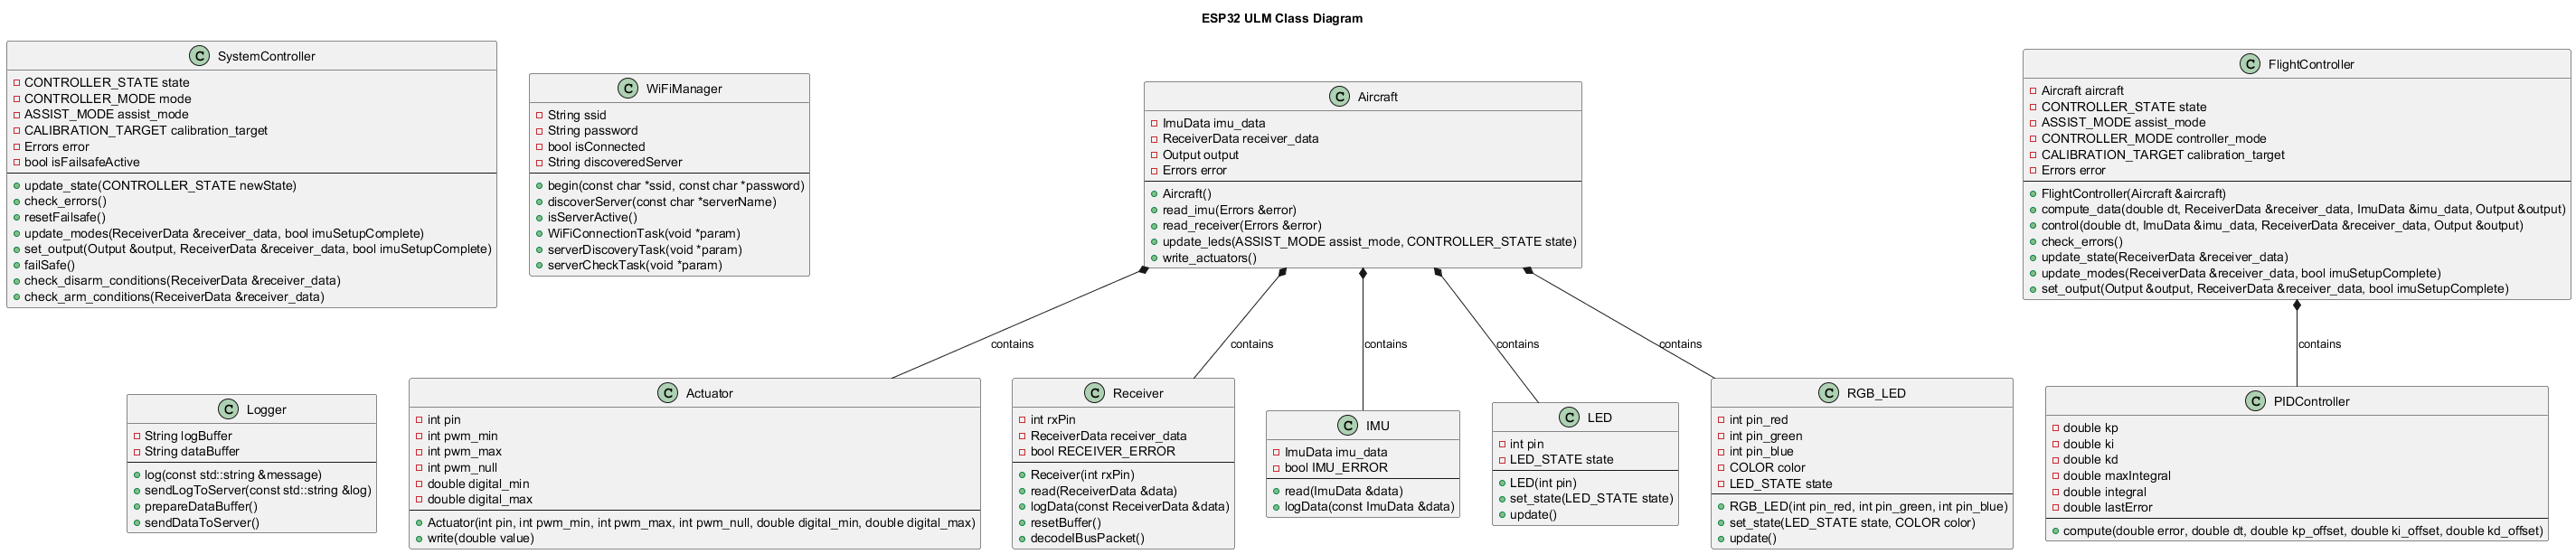
\includegraphics[width=\textwidth]{diagrams/esp32_class_diagram.png}
    \caption{Diagramma UML delle classi del Flight Controller (ESP32).}
    \label{fig:esp32_class_diagram}
\end{figure}

\begin{figure}[h!]
    \centering
    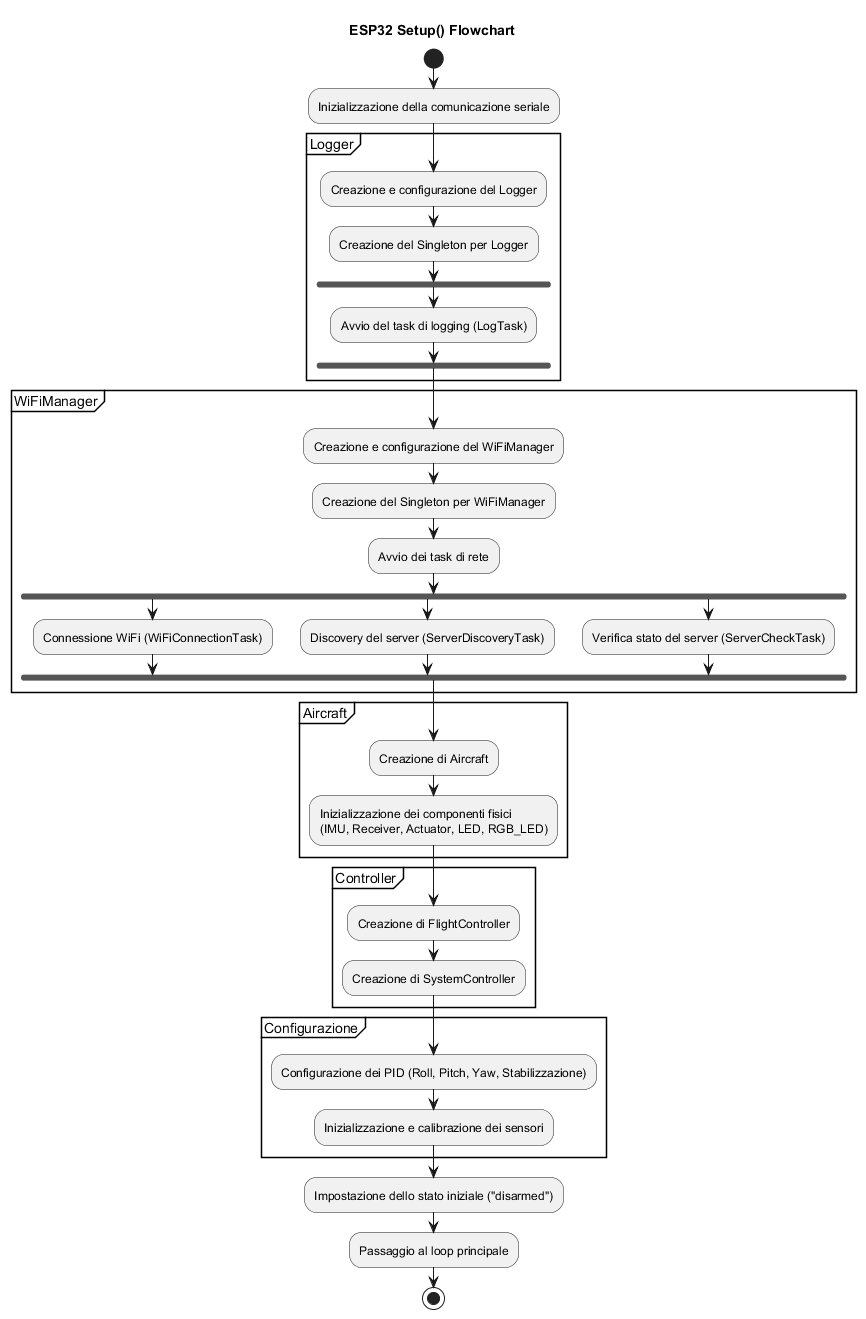
\includegraphics[width=\textwidth]{diagrams/esp32_setup_flowchart.png}
    \caption{Diagramma di flusso della configurazione iniziale del Flight Controller.}
    \label{fig:esp32_setup_flowchart}
\end{figure}

\begin{figure}[h!]
    \centering
    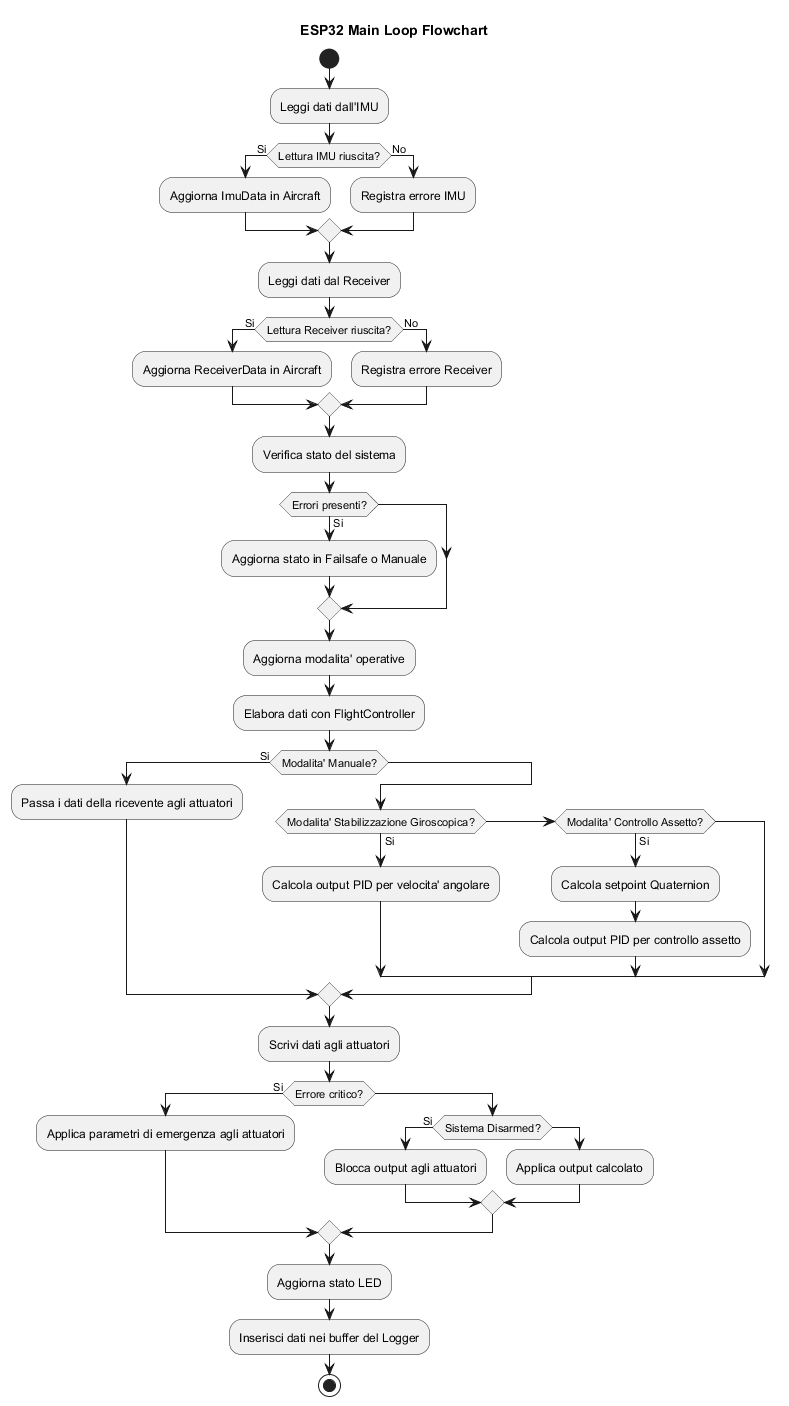
\includegraphics[width=\textwidth]{diagrams/esp32_loop_flowchart.png}
    \caption{Diagramma di flusso del loop principale del Flight Controller.}
    \label{fig:esp32_loop_flowchart}
\end{figure}


\begin{figure}[h!]
    \centering
    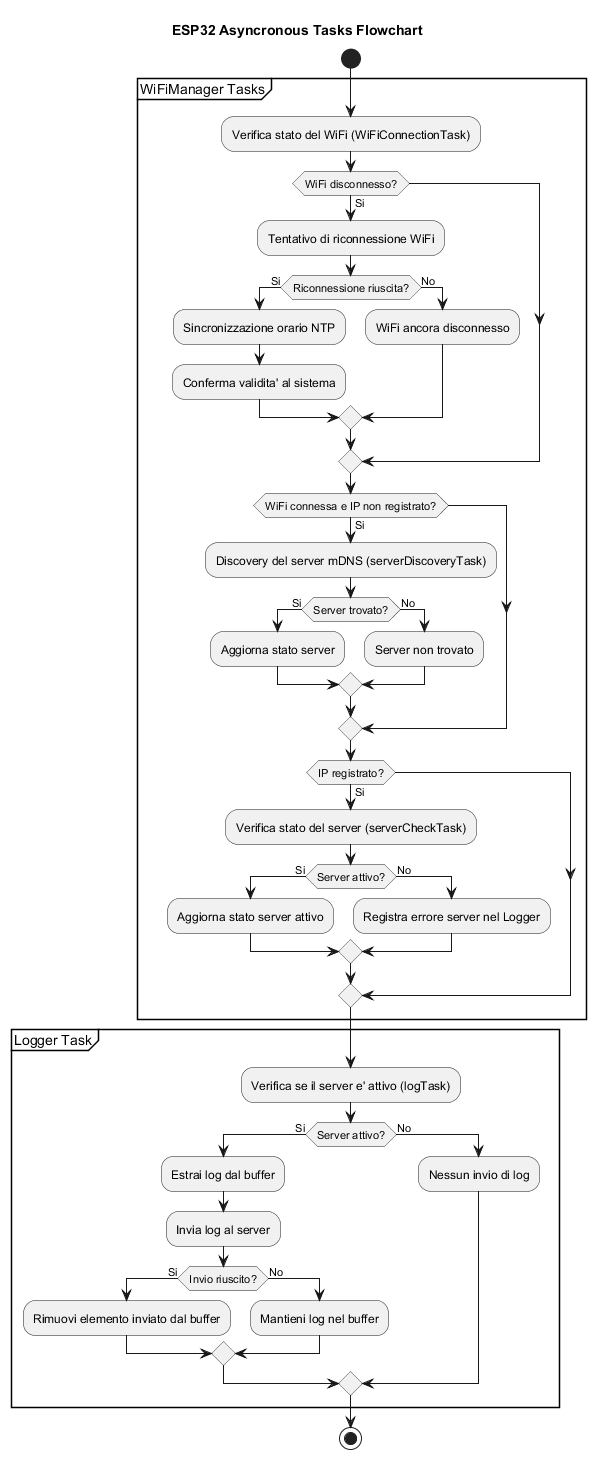
\includegraphics[width=\textwidth]{diagrams/esp32_asynctasks_flowchart.png}
    \caption{Diagramma di flusso dei task asincroni del Flight Controller.}
    \label{fig:esp32_asynctasks_flowchart}
\end{figure}